\section{CVE-2025-23266 --- Technical Analysis}
\label{sec:vuln}

% ~6.000 characters total across subsections

\subsection{Vulnerability Description}
\label{subsec:vuln-desc}

CVE-2025-23266 is a \textbf{container escape vulnerability} in the NVIDIA Container Toolkit \cite{nvd_cve_2025_23266, nvidia_advisory_2025}. It was publicly disclosed in 2025 and assigned a CVSS v3.1 base score of \textbf{9.0 (Critical)} \cite{cvss_v31_spec}, reflecting the combination of high confidentiality, integrity, and availability impact at the host level, with the attack vector being local (within the container) but resulting in complete host compromise.

The vulnerability affects versions of the NVIDIA Container Toolkit prior to the patched release and stems from a failure to sanitise the execution environment of the \texttt{nvidia-ctk} OCI hook process. Specifically, environment variables set within the container — including \texttt{LD\_PRELOAD} — are inherited by the hook process when it is invoked by the container runtime on the host. Since the hook process runs with root privileges on the host, this inheritance allows an attacker inside the container to force the loading of an arbitrary shared library into the host's privileged process space.

\begin{infobox_env}
CVE-2025-23266 does not require any kernel vulnerability, any special container privileges (e.g., \texttt{--privileged}), or any network access. The only prerequisite is that the attacker can run a container on a host equipped with the NVIDIA Container Toolkit (a standard precondition in any GPU cloud environment).
\end{infobox_env}

Graphically we can represent the attack flow as follows:


\begin{figure}[htbp]
  \centering
  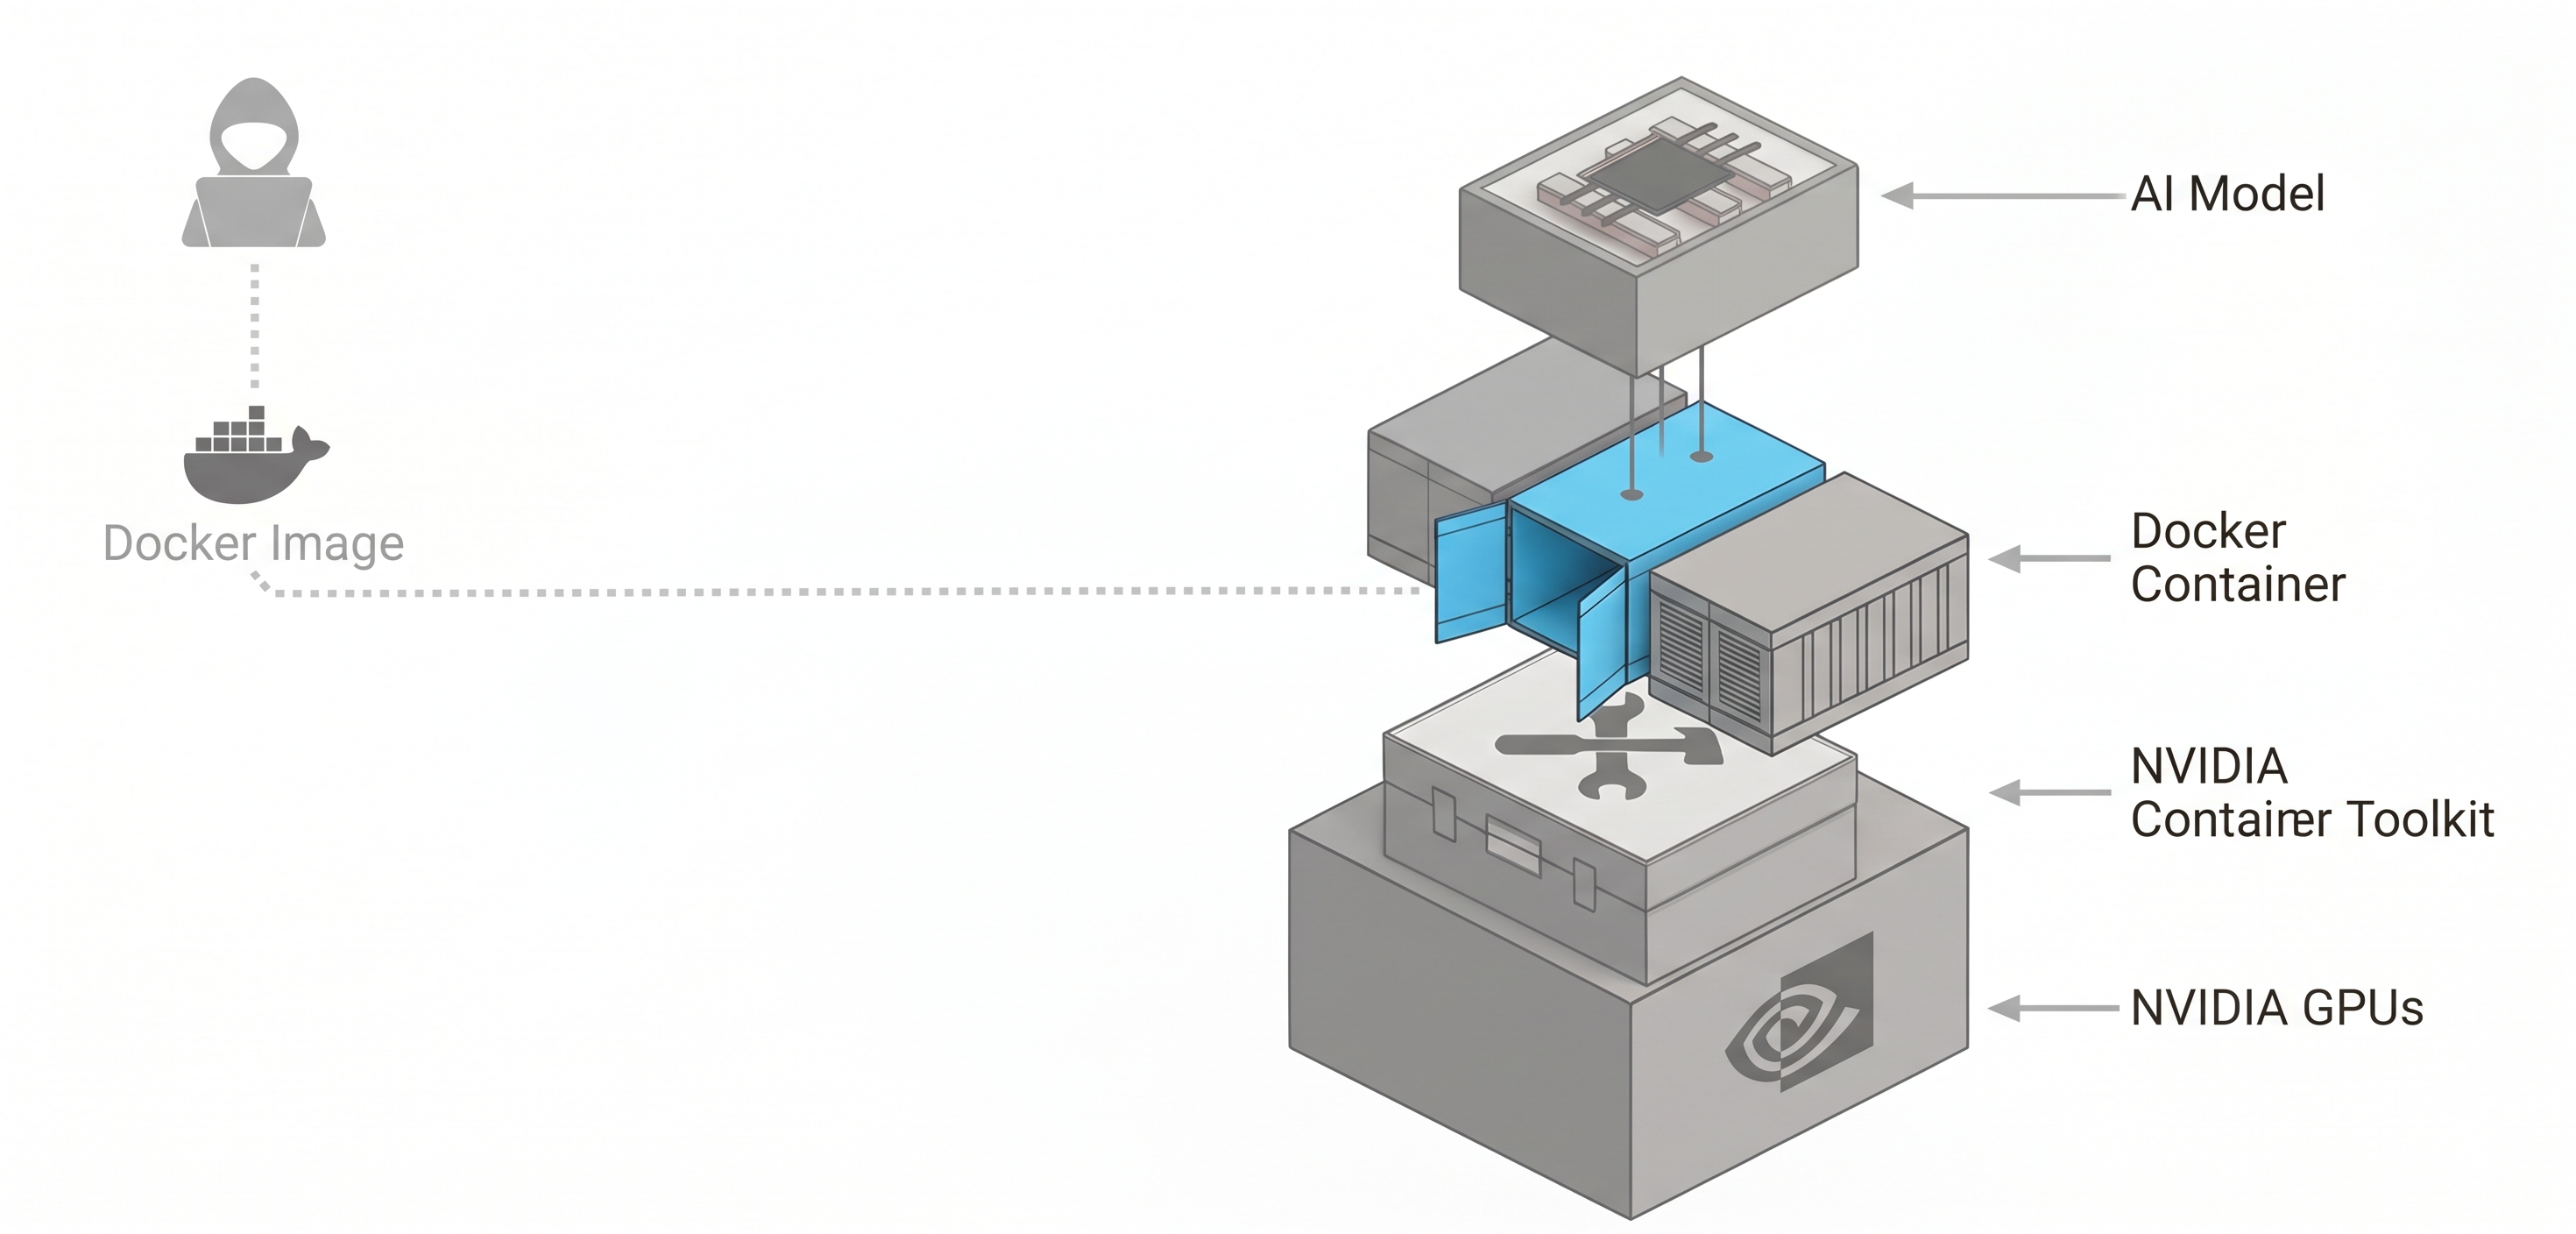
\includegraphics[width=\textwidth]{images/nvidiacontainer.png}
  \caption{NVIDIA Container Toolkit architecture and hook execution flow.}
  \label{fig:nvidia-container}
\end{figure}


\subsection{Root Cause: Unsafe Environment Inheritance}
\label{subsec:root-cause}

To understand the root cause precisely, we must examine how the OCI hook is invoked. When a container with GPU access is started, the container runtime (e.g., \texttt{runc} or \texttt{containerd}) reads the container's OCI bundle specification (\texttt{config.json}), which includes a list of hooks. The NVIDIA prestart hook entry looks approximately as follows:

\begin{lstlisting}[language=bash, caption={Simplified OCI hook specification for nvidia-ctk (config.json excerpt).}]
"hooks": {
  "prestart": [
    {
      "path": "/usr/bin/nvidia-ctk",
      "args": ["nvidia-ctk", "runtime", "hook", "prestart"],
      "env": []
    }
  ]
}
\end{lstlisting}

The OCI runtime specification states that hook processes receive the container's environment in the \texttt{env} field of the hook configuration. However, the problematic behaviour in the vulnerable versions of the toolkit arises from the fact that the hook process additionally inherits environment variables from its parent process (and the parent process's environment is populated, directly or indirectly, from the container's configured environment variables).
 
The crucial flaw is the absence of an explicit \texttt{execve()} call with a sanitised, minimal environment array before the hook begins its privileged operations \cite{linux_execve_manpage}. In Unix process semantics, \texttt{execve()} is the mechanism by which a process can replace its image with a new executable; critically, it accepts an explicit \texttt{envp} array, allowing the caller to specify a completely controlled environment for the new process. A correctly written privileged process that must execute in an environment derived from untrusted input would call \texttt{execve()} with a hand-crafted, minimal \texttt{envp} containing only the variables strictly necessary for operation.

The vulnerable toolkit does not perform this sanitisation. The \texttt{LD\_PRELOAD} variable, if present in the container's environment, propagates to the hook process where the dynamic linker acts upon it faithfully \cite{linux_ldso_manpage} (loading the attacker-specified library with root privileges).

\subsection{Attack Surface and Preconditions}
\label{subsec:attack-surface}

The attack surface of CVE-2025-23266 is defined by the following preconditions:

\begin{enumerate}
  \item \textbf{Vulnerable toolkit version}: The host must be running a version of the NVIDIA Container Toolkit prior to the patch. This affects a wide range of deployments that have not applied the security update.
  \item \textbf{GPU-enabled container}: The attacker must be able to start a container with GPU access (e.g., using the \texttt{-{}-gpus} flag in Docker or the \texttt{nvidia.com/gpu} resource request in Kubernetes). In shared cloud environments, this is a standard capability offered to paying customers.
  \item \textbf{Ability to set environment variables}: The attacker must be able to define environment variables for their container. This is universally true for any container a user controls.
  \item \textbf{Writable shared path}: The attacker's malicious shared library must be accessible to the host-side linker. This is achieved by placing the library in a path that is shared between the container and the host (such as a mounted volume or a device path accessible from both).
\end{enumerate}
 
Notably absent from this list are: kernel exploits, elevated container capabilities, network access, and any form of social engineering. The attack is self-contained within the container startup sequence.

\subsection{Exploit Walkthrough}
\label{subsec:exploit-walkthrough}

The following provides a conceptual, step-by-step walkthrough of the exploit chain.

\begin{enumerate}
  \item \textbf{Craft the malicious shared library.} The attacker writes a shared library containing a constructor function (a function annotated with \texttt{\_\_attribute\_\_((constructor))} in C) that executes the attacker's payload when the library is loaded. Because this runs before \texttt{main()}, it executes at the earliest possible moment in the host process lifecycle, before any security checks in the hook's application logic.
 
\begin{lstlisting}[language=C, caption={Pseudocode for the malicious shared library constructor.}]
// evil.c -- compiled to evil.so
#include <unistd.h>
#include <stdlib.h>
 
__attribute__((constructor))
void payload(void) {
    // Executed with root privileges on the HOST
    // at the moment the hook process loads this library.
    // Example: spawn a reverse shell, write an SSH key,
    // create a SUID shell binary, etc.
    system("/bin/bash -c 'cp /bin/bash /tmp/rootshell"
           " && chmod u+s /tmp/rootshell'");
}
\end{lstlisting}
 
  \item \textbf{Place the library on a shared path.} The library must be reachable from the host filesystem at the time the hook runs. The attacker mounts a host directory into their container (a common practice for data I/O) and writes the compiled \texttt{evil.so} there. Alternatively, certain NVIDIA device paths mounted by the toolkit itself may be exploitable.
 
  \item \textbf{Set \texttt{LD\_PRELOAD} in the container environment.} When starting the container, the attacker sets the environment variable \texttt{LD\_PRELOAD} to the host-side path of \texttt{evil.so}. In Docker CLI syntax:
 
\begin{lstlisting}[language=bash, caption={Container launch with injected LD\_PRELOAD.}]
docker run --gpus all \
  -e LD_PRELOAD=/mnt/shared/evil.so \
  -v /host/shared:/mnt/shared \
  attacker-image
\end{lstlisting}
 
  \item \textbf{Hook invocation.} As part of the container startup sequence, the OCI runtime invokes the NVIDIA prestart hook (\texttt{nvidia-ctk runtime hook prestart}) on the host with root privileges. Due to the environment inheritance vulnerability, \texttt{LD\_PRELOAD=/mnt/shared/evil.so} is present in the hook's environment.
 
  \item \textbf{Dynamic linker loads the malicious library.} The host's dynamic linker reads \texttt{LD\_PRELOAD} and maps \texttt{evil.so} into the hook process's address space before any standard libraries. The constructor function executes immediately.
 
  \item \textbf{Arbitrary code runs as root on the host.} The attacker's payload runs with the full privileges of the hook process (root on the host) achieving a complete container escape. The container itself need not even finish starting for the escape to succeed.
\end{enumerate}

The elegance of this exploit chain is its simplicity. No memory corruption, no kernel exploit, no race condition. A single environment variable and a compiled shared library are sufficient to escape the container and own the host.